
\documentclass[12pt,a4paper]{article}

% ---- Packages ----
\usepackage[margin=1in]{geometry}
\usepackage{graphicx}
\usepackage{float}
\usepackage{booktabs}
\usepackage{longtable}
\usepackage{array}
\usepackage{titlesec}
\usepackage{hyperref}
\usepackage{xcolor}
\usepackage{setspace}
\usepackage{fancyhdr}
\usepackage{caption}
\usepackage{subcaption}
\usepackage{amsmath, amssymb}
\usepackage{enumitem}
\usepackage{tcolorbox}
\usepackage{listings}
\usepackage{tikz}
\usepackage{pgfplots}
\pgfplotsset{compat=1.18}

% ---- Colors & Hyperref ----
\definecolor{primary}{HTML}{0F766E} % teal
\definecolor{accent}{HTML}{2563EB}  % blue
\definecolor{light}{HTML}{F1F5F9}   % slate-50
\definecolor{dark}{HTML}{0B1220}    % dark text

\hypersetup{
  colorlinks=true,
  linkcolor=primary,
  urlcolor=accent,
  citecolor=primary
}

% ---- Section Formatting ----
\titleformat{\section}{\Large\bfseries\color{primary}}{}{0em}{}
\titleformat{\subsection}{\large\bfseries\color{primary}}{}{0em}{}
\titleformat{\subsubsection}{\normalsize\bfseries\color{primary}}{}{0em}{}

% ---- Header / Footer ----
\pagestyle{fancy}
\fancyhf{}
\lhead{\textit{Comparative Study of Sorting Algorithms}}
\rhead{\thepage}
\renewcommand{\headrulewidth}{0.4pt}

% ---- Code Styling ----
\lstdefinestyle{code}{
  basicstyle=\ttfamily\small,
  backgroundcolor=\color{light},
  frame=single,
  rulecolor=\color{light},
  keywordstyle=\color{accent}\bfseries,
  commentstyle=\color{primary},
  stringstyle=\color{accent},
  numbers=left,
  numberstyle=\tiny,
  stepnumber=1,
  numbersep=8pt,
  showstringspaces=false,
  tabsize=2,
  breaklines=true
}

% ---- Convenience Macros ----
\newcommand{\algoname}[1]{\textbf{#1}}
\newcommand{\theotabname}{Theoretical Time and Space Complexities of Sorting Algorithms}

% ---- Document ----
\begin{document}
\onehalfspacing

% ---- Title Page ----
\begin{titlepage}
\centering
\vspace*{2cm}
{\Huge\bfseries Comparative Study and Complexity Analysis of Sorting Algorithms\par}
\vspace{1cm}
{\Large DAA SEC-R \par}
\vspace{0.75cm}
\begin{tcolorbox}[colback=light,colframe=primary,boxrule=0.6pt,arc=2mm,width=0.9\textwidth]
\centering
\begin{tabular}{@{}ll@{}}
\textbf{Student Name:} & Your Name Here \\
\textbf{Roll No.:} & 000000 \\
\textbf{Course:} & Design and Analysis of Algorithms \\
\textbf{Instructor/Guide:} & Prof.~Name Here \\
\textbf{Institution:} & College/University Name \\
\textbf{Submission Date:} & \today \\
\end{tabular}
\end{tcolorbox}

\vfill
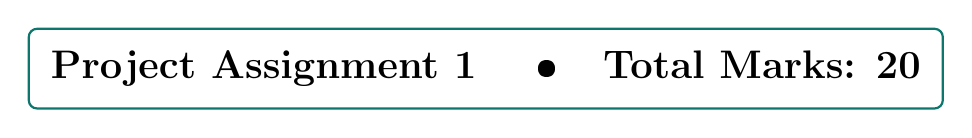
\begin{tikzpicture}
\node[draw=primary,rounded corners=3pt,thick,inner sep=8pt] (A) at (0,0) {\Large\bfseries Project Assignment 1 \quad\textbullet\quad Total Marks: 20};
\end{tikzpicture}

\vspace*{1cm}
\end{titlepage}

% ---- Front Matter ----
\pagenumbering{roman}
\begin{abstract}
\noindent
This report presents a comparative study of classic and advanced sorting algorithms with both theoretical and experimental analysis.
We implement multiple sorting strategies, evaluate their time--space complexities, and measure performance over a diverse range of input sizes and data characteristics.
Our experiments include robustness checks (multiple trials per setting) and controlled hardware/software configuration notes to ensure reproducibility.
\end{abstract}

\tableofcontents
\listoffigures
\listoftables
\clearpage
\pagenumbering{arabic}

% ---- Objective ----
\section{Objective}
\begin{tcolorbox}[colback=light,colframe=primary,boxrule=0.6pt,arc=2mm]
\textbf{Goal: } Design, implement, and analyze various sorting algorithms, comparing their \emph{theoretical} and \emph{experimental} time complexities under different input sizes and data characteristics.
\end{tcolorbox}

% ---- Algorithms Implemented ----
\section{Algorithms Implemented}
\begin{enumerate}[leftmargin=2em,label=\arabic*.]
  \item Bubble Sort
  \item Selection Sort
  \item Insertion Sort
  \item Merge Sort
  \item Quick Sort (deterministic and randomized)
  \item Heap Sort
  \item Counting Sort
  \item Radix Sort
  \item Bucket Sort
\end{enumerate}
\noindent
\textit{(Optional extensions: Shell Sort, TimSort, IntroSort.)}

% ---- Theoretical Complexity ----
\section{Theoretical Complexity Analysis}
\begin{table}[H]
\centering
\caption{\theotabname}
\label{tab:theoretical-complexities}
\begin{tabular}{@{}lcccc@{}}
\toprule
\textbf{Algorithm} & \textbf{Best} & \textbf{Average} & \textbf{Worst} & \textbf{Space} \\
\midrule
Bubble Sort     & $O(n)$          & $O(n^2)$         & $O(n^2)$       & $O(1)$ \\
Selection Sort  & $O(n^2)$        & $O(n^2)$         & $O(n^2)$       & $O(1)$ \\
Insertion Sort  & $O(n)$          & $O(n^2)$         & $O(n^2)$       & $O(1)$ \\
Merge Sort      & $O(n\log n)$    & $O(n\log n)$     & $O(n\log n)$   & $O(n)$ \\
Quick Sort      & $O(n\log n)$    & $O(n\log n)$     & $O(n^2)$       & $O(\log n)$ \\
Heap Sort       & $O(n\log n)$    & $O(n\log n)$     & $O(n\log n)$   & $O(1)$ \\
Counting Sort   & $O(n+k)$        & $O(n+k)$         & $O(n+k)$       & $O(k)$ \\
Radix Sort      & $O(nk)$         & $O(nk)$          & $O(nk)$        & $O(n+k)$ \\
Bucket Sort     & $O(n+k)$        & $O(n+k)$         & $O(n^2)$       & $O(n)$ \\
\bottomrule
\end{tabular}
\end{table}

% ---- Experimental Setup ----
\section{Experimental Setup}
\subsection{Hardware / Software Configuration}
\begin{table}[H]
\centering
\caption{System Specifications (Update as appropriate)}
\label{tab:system-specs}
\begin{tabular}{@{}ll@{}}
\toprule
\textbf{Processor} & Intel Core i9-14900HX (24 cores) \\
\textbf{RAM} & 32 GB DDR5 \\
\textbf{Storage} & NVMe SSD \\
\textbf{Operating System} & Windows 11 Pro / Linux (kernel version) \\
\textbf{Language / Tools} & Python 3.12 with \texttt{time}/\texttt{perf\_counter}, Matplotlib; or C/C++ with \texttt{chrono} \\
\bottomrule
\end{tabular}
\end{table}

\subsection{Input Sizes and Data Distributions}
We evaluate input sizes $n \in \{100, 500, 1000, 5000, 10^4, 5\times10^4, 10^5, 5\times10^5, 10^6, 5\times10^6, 10^7\}$ under:
\begin{itemize}[leftmargin=2em]
  \item Random (uniform) data
  \item Sorted data (best case for some algorithms)
  \item Reverse-sorted data (worst case for some algorithms)
\end{itemize}

\subsection{Measurement Methodology}
For each algorithm and input size, we perform $T=5$ independent trials, recording elapsed time using a high-resolution clock and reporting the \emph{mean} runtime.
We also compute the \emph{standard deviation} as a measure of dispersion.

% ---- Robustness ----
\section{Robustness}
All experiments are repeated multiple times under identical conditions to ensure accuracy, consistency, and dependability. Robustness quantifies how consistently runtime performance holds up over multiple trials and confirms that minor changes in the environment or system load have negligible impact on outcomes.

% ---- Implementation Notes ----
\section{Implementation Notes}
\subsection{Design Guidelines}
\begin{itemize}[leftmargin=2em]
  \item Modular functions per algorithm with clear docstrings/comments.
  \item Reproducible random seeds for data generation.
  \item Avoid unnecessary copying of arrays to minimize measurement noise.
  \item Warm-up runs to reduce one-time overheads (e.g., JIT/cache effects).
\end{itemize}

\subsection{Pseudocode Examples}
\paragraph{Insertion Sort}
\begin{lstlisting}[style=code,language=C,caption={Insertion Sort (pseudocode)}]
void insertionSort(int A[], int n) {
    for (int i = 1; i < n; i++) {
        int key = A[i];
        int j = i - 1;
        while (j >= 0 && A[j] > key) {
            A[j + 1] = A[j];
            j--;
        }
        A[j + 1] = key;
    }
}
\end{lstlisting}

\paragraph{Merge Sort (Top-Down)}
\begin{lstlisting}[style=code,language=C,caption={Merge Sort (pseudocode)}]
void merge(int A[], int l, int m, int r) { /* ... */ }

void mergeSort(int A[], int l, int r) {
    if (l >= r) return;
    int m = l + (r - l) / 2;
    mergeSort(A, l, m);
    mergeSort(A, m + 1, r);
    merge(A, l, m, r);
}
\end{lstlisting}

\paragraph{Quick Sort (Randomized Pivot)}
\begin{lstlisting}[style=code,language=C,caption={Quick Sort with Random Pivot (pseudocode)}]
int partition(int A[], int l, int r) { /* ... */ }

void quickSort(int A[], int l, int r) {
    if (l >= r) return;
    int p = l + rand() % (r - l + 1);
    swap(A[p], A[r]);
    int q = partition(A, l, r); // final pivot index
    quickSort(A, l, q - 1);
    quickSort(A, q + 1, r);
}
\end{lstlisting}

% ---- Results Templates ----
\section{Results}
\subsection{Runtime Tables (Template)}
% Example longtable template for results; duplicate per algorithm if needed
\begin{longtable}{@{}lrrrrr@{}}
\caption{Example: Insertion Sort Runtime (ms) across Trials and Mean/Std}\label{tab:ins-results}\\
\toprule
\textbf{n} & \textbf{Trial 1} & \textbf{Trial 2} & \textbf{Trial 3} & \textbf{Trial 4} & \textbf{Trial 5} \\
\midrule
\endfirsthead
\toprule
\textbf{n} & \textbf{Trial 1} & \textbf{Trial 2} & \textbf{Trial 3} & \textbf{Trial 4} & \textbf{Trial 5} \\
\midrule
\endhead
100   &   &   &   &   &   \\
500   &   &   &   &   &   \\
1000  &   &   &   &   &   \\
5000  &   &   &   &   &   \\
10000 &   &   &   &   &   \\
\bottomrule
\end{longtable}

\subsection{Graphs: Theory vs Experiment}
\noindent Place exported PNG/PDF graphs in the project folder and include them as below.
\begin{figure}[H]
\centering
\includegraphics[width=0.85\textwidth]{fig_merge_sort.png}
\caption{Merge Sort: Theoretical trend ($O(n\log n)$) vs experimental data points.}
\label{fig:merge-graph}
\end{figure}

\begin{figure}[H]
\centering
\includegraphics[width=0.85\textwidth]{fig_quick_sort.png}
\caption{Quick Sort (randomized): Theoretical trend vs experimental data points.}
\label{fig:quick-graph}
\end{figure}

\subsection{Optional: Direct PGFPlots Example}
\noindent Alternatively, you can plot small datasets directly in \LaTeX:
\begin{figure}[H]
\centering
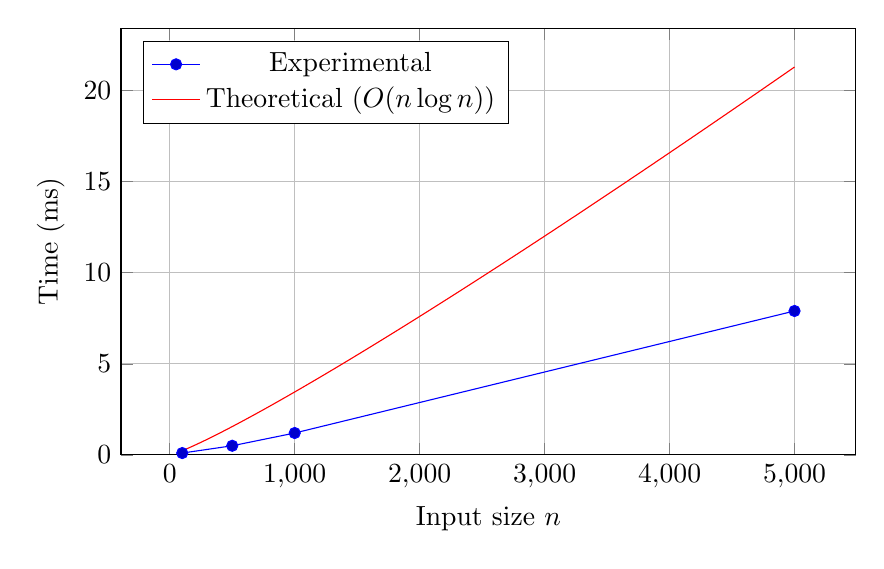
\begin{tikzpicture}
\begin{axis}[
    width=0.9\textwidth,
    height=7cm,
    xlabel={Input size $n$},
    ylabel={Time (ms)},
    ymin=0,
    grid=both,
    legend pos=north west
]
\addplot coordinates {(100,0.1) (500,0.5) (1000,1.2) (5000,7.9)};
\addlegendentry{Experimental}
\addplot+[mark=none,domain=100:5000,samples=100] {0.0005*x*ln(x)};
\addlegendentry{Theoretical ($O(n\log n)$)}
\end{axis}
\end{tikzpicture}
\caption{Example PGFPlots: Merge Sort trend illustration (replace with real data).}
\end{figure}

% ---- Discussion & Analysis ----
\section{Discussion}
\subsection{Observed Trends}
\begin{itemize}[leftmargin=2em]
  \item Divide-and-conquer algorithms (Merge, Quick, Heap) scale better than quadratic sorts for $n \ge 10^4$.
  \item Quick Sort with randomized pivot is competitive; however, worst-case spikes may appear for adversarial inputs.
  \item Linear-time sorts (Counting, Radix, Bucket) excel when assumptions about key ranges and distributions hold.
\end{itemize}

\subsection{When Theory Diverges from Practice}
\begin{itemize}[leftmargin=2em]
  \item Constant factors, cache behavior, and implementation details can favor simpler algorithms on small $n$.
  \item Memory allocation and recursion overhead impact Merge/Quick.
  \item Python vs C/C++ runtime differences due to interpreter/optimizer effects.
\end{itemize}

% ---- Conclusion ----
\section{Conclusion and Future Scope}
\textbf{Conclusion.} For small datasets (e.g., $n \le 10^3$), insertion sort can be competitive due to low overhead. For medium to large datasets, $O(n\log n)$ sorts dominate, with merge sort and randomized quick sort showing consistent performance. When applicable, counting/radix methods achieve near-linear behavior.
\\[0.5em]
\textbf{Future Scope.} Explore hybrid strategies (e.g., using insertion sort on small partitions), adaptive algorithms (TimSort), and parallel implementations leveraging multicore CPUs/GPUs.

% ---- Submission Requirements ----
\section{Submission Requirements}
\begin{itemize}[leftmargin=2em]
  \item \textbf{Source Code} with comments and modular design.
  \item \textbf{Short Report (4--6 pages)} including: problem description, algorithms \& pseudocode, time/space analysis, experimental setup \& results, conclusion \& future scope.
  \item \textbf{Graphs/Charts} comparing performance across input sizes and data distributions.
  \item \textbf{Viva Preparation} based on algorithmic design principles and trade-offs.
\end{itemize}

% ---- Marking Rubric ----
\section{Evaluation Rubric (As Provided)}
\begin{table}[H]
\centering
\caption{Grading Criteria Summary}
\begin{tabular}{@{}lcr@{}}
\toprule
\textbf{Criteria} & \textbf{Description} & \textbf{Marks} \\
\midrule
Algorithm Design \& Implementation & Correctness and efficiency of code & 6 \\
Complexity Analysis & Theoretical + experimental comparisons & 4 \\
Documentation \& Report & Clarity, pseudocode, results discussion & 4 \\
Viva / Presentation & Understanding of design, performance, trade-offs & 6 \\
\midrule
\textbf{Total} & & \textbf{20} \\
\bottomrule
\end{tabular}
\end{table}

% ---- Viva Hints ----
\section{Viva Hints}
\begin{itemize}[leftmargin=2em]
  \item Explain why $O(n\log n)$ beats $O(n^2)$ and when linear-time sorts apply.
  \item Discuss pivot selection strategies and stability of algorithms.
  \item Comment on memory usage (in-place vs auxiliary arrays).
  \item Describe robustness methodology and reproducibility.
\end{itemize}

% ---- References ----
\section{References}
\begin{enumerate}[leftmargin=2em]
  \item Cormen, Leiserson, Rivest, Stein. \textit{Introduction to Algorithms}, MIT Press.
  \item Sedgewick, Wayne. \textit{Algorithms}, Addison-Wesley.
  \item Official Python and C++ documentation for timing utilities.
\end{enumerate}

\end{document}
